\documentclass[12pt,landscape]{exam}
\usepackage[
  margin=.4in
]{geometry}
\usepackage[per-mode=symbol]{siunitx}
\usepackage{enumitem,multicol,tikz}


\begin{document}
\pagestyle{empty}

\newcommand{\mycontent}{
  \subsection*{Newton's First Law}
  \hrule

  \vspace{1em}
  An object \fillin[continues][12em] in its state of rest or uniform speed in a straight line unless acted on by a \fillin[net force][12em].


  \vspace{1em}

  \subsection*{Newton's Second Law}
  \hrule

  \vspace{1em}
  Acceleration is
  
  \begin{itemize}
    \item \fillin[directly proportional][15em] to net force,
    \item in the \fillin[same direction][15em] as net force, and
    \item \fillin[inversely proportional][15em] to mass.
  \end{itemize}

  \noindent
  Two Equations:

  \vspace{2em}

  \subsection*{Newton's Third Law}
  \hrule

  \vspace{2em}
  If a first object puts a force on a second object, then the second object puts an \fillin[equal][7em] and \fillin[opposite][7em] force on the first object.

  \vspace{1em}

  \noindent
  \emph{``Every \fillin[action force][12em] has an \fillin[equal][7em] and \fillin[opposite][7em] reaction force.''}

  \begin{tikzpicture}
    \def\sep{4}
    \path (0,0) node[anchor=west] {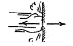
\includegraphics{../../images/fist.png}}
      ++(0,-1.5) node[anchor=west] {\small\bf Action:}
      +(0,-.5) node[anchor=west] {\footnotesize\emph{fist hits wall}} 
      ++(0,-1.2) node[anchor=west] {\small\bf Reaction:} ;
    % \path (\sep,0) node[anchor=west] {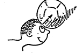
\includegraphics{../../images/soccer.png}}
    %   ++(0,-1.5) node[anchor=west] {\small\bf Action:}
    %   +(0,-.5) node[anchor=west] {\footnotesize\emph{head hits ball}} 
    %   ++(0,-1.2) node[anchor=west] {\small\bf Reaction:} ;
    \path (\sep,0) node[anchor=west] {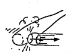
\includegraphics{../../images/bat.png}}
      ++(0,-1.5) node[anchor=west] {\small\bf Action:}
      +(0,-.5) node[anchor=west] {\footnotesize\emph{bat hits ball}} 
      ++(0,-1.2) node[anchor=west] {\small\bf Reaction:} ;
    \path (2*\sep,0) node[anchor=west] {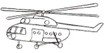
\includegraphics{../../images/helicopter.jpg}}
      ++(0,-1.5) node[anchor=west] {\small\bf Action:}
      +(0,-.5) node[anchor=west] {\footnotesize\emph{rotors push air $\downarrow$}} 
      ++(0,-1.2) node[anchor=west] {\small\bf Reaction:} ;
  \end{tikzpicture}

}

\setlength{\columnsep}{.8in}
\begin{multicols}{2}

  \mycontent

  \columnbreak

  \mycontent
\end{multicols}



\end{document}